%!TEX encoding = UTF-8 Unicode
%!TEX program = xelatex

\documentclass[bachelor]{ustcthesis}
% bachelor|master|doctor
\usepackage{ustcextra}
\graphicspath{{figures/}}
\bibliographystyle{ustcauthoryear}
% \bibliographystyle{ustcnumerical}

\newcommand{\makevector}[1]{{\mathbf #1}}
\newcommand{\vvec}{{\makevector{v}}}
\newcommand{\vecc}{{\makevector{c}}}
\newcommand{\mydash}{\raisebox{0.5mm}{------}}

\title{词向量嵌入模型的分析,\\改进与应用}
\author{刘力源}
\major{计算机科学与技术}
\advisor{宋睿华, 徐林莉}
\submitdate{二〇一六年六月}
%\secrettext{机密\quad 小于等于20年}   % 内部|秘密|机密,注释本行则不保密
\depart{11系}

\entitle{Analysis, reinforcement and application of Word Embedding}
\enauthor{Liyuan Liu}
\enmajor{Computer Science and Technology}
\enadvisor{Ruihua Song, Linli Xu}
\ensubmitdate{June, 2016}
%\ensecrettext{Confidential\quad Less than or equal to 20 years}  % Internal|Secret|Confidential

\begin{document}

\maketitle

%
% 本科论文:
%   frontmatter: 致谢、目录、中文摘要、英文摘要
%   mainmatter: 正文章节、参考文献
%   appendix: 附录
%
% 硕博论文:
%   frontmatter: 中文摘要、英文摘要、目录、符号说明
%   mainmatter: 正文、参考文献
%   appendix: 附录
%   backmatter: 致谢、发表论文
%

\frontmatter
\begin{abstract}

在自然语言处理(Natural Language Processing)领域,一个基础性的受到全世界学者广泛关注的问题是如何能合理地表示词语。近几年来,\emph{word2vec}及其相关的一系列工作通过词向量嵌入的方法(Word Embedding)在这一问题上取得了突破性的成果,也使得词向量嵌入的模型成为了研究的热点。本文对现有的词向量嵌入模型进行了总结与分析,对词向量的性质进行了分析与讨论,然后基于这些模型的一些缺点, 如无法很好地判断和处理多义词,对模型进行了改进,并通过实验对改进后的模型进行了验证,说明了改进的有效性。

\keywords{自然语言处理\zhspace{} 词向量嵌入\zhspace{} 多义词}
\end{abstract}

\begin{enabstract}

The task of representing words, known as Word Representation or Word Embedding, is one of the major topics in Natural Language Processing. With the recent advances like the \emph{word2vec} toolbox, how to representing words or phrases as vectors of real numbers in a low-dimensional space has received a significant amount of attention. In this paper, we summarize and analyze several popular word embedding models, improve word representation to overcome former drawbacks, such as the lack of method to judge and deal with polysemy. Extensive experimental results demonstrates the effective of proposed method.

\enkeywords{Natural Language Processing, Word Embedding, Polysemy}
\end{enabstract}

\tableofcontents
\listoffigures
\listoftables
% \listofalgorithms  % 算法索引,如不需要,可直接注释掉本行
% \input{chapters/notation}

\mainmatter
\iffalse

\bibliography{..\\bib\\tex.bib}

\fi

\chapter{引言}
\label{chap:intro}
文本数据是机器学习,数据挖掘,自然语言处理等领域所经常需要处理的一种数据形式。在处理文本数据时,常常所要面对的一个问题就是应该如何表示词语。为了解决这个问题,一种常用的方法是,使用一种只有一个维度的值为1其余维度的值均为0的向量来表示值为1的维度的编号所对应的词语,例如,使用$[1, 0, ..., 0]$表示字典中的第一个词语(这种向量也被称为one-hot 向量)。这种方法非常直观,但由于字典中往往会包括多达几万个不同词语,one-hot向量往往会有较大的维度,而使得模型的训练变得较为困难。另一方面,这种方法,如同大多数传统的方法一样,忽略了词语的语义和语法层面的信息与关系。

\citep{rumelhart1988learning}第一次提出了词向量的概念。词向量是一种类似于one-hot向量的使用向量来表示词语的方法。但与one-hot向量所不同的是,词向量没有将向量限制为某种特殊的向量,而是使用维度不高的实数空间上的一般向量来表示词语。这种做法较one-hot向量而言,具有较小的向量维度。同时,由于词向量不是由人工设定的方式生成的,而是根据文本的特点通过学习自动生成的,词向量也会携带一部分词语的语义与语法信息。这些特性,使得词向量的概念一经提出,就迅速被广泛运用到神经网络语言模型等许多自然语言处理的问题中,并取得了可观的成功\citep{collobert2008unified,schwenk2007continuous}。

几年前,Google 发布了著名的\emph{word2vec}工具包,这个工具包训练得到的词向量不光具有维度低的特点,还具有一些非常有趣的特性\citep{mikolov2013efficient,mikolov2013distributed,mikolov2013linguistic}。一方面,\emph{word2vec}可以在较大量的语料上以较高效率学习并获得具有较高质量的词向量。这种高效性使得它可以被广泛地运用在各种模型中。除此之外,更引人注意的是,通过这个模型学习出的词向量可以通过向量的加减运算来表示词语间的语义语法关系。比如说,如果我们用$\vvec[\mbox{词语}]$表示一个词语所对应的词向量,我们会发现存在如下关系:$\vvec[\mbox{man}]-\vvec[\mbox{woman}] \approx \vvec[\mbox{king}] - \vvec[\mbox{queen}]$,$\vvec[\mbox{Chinese}] + \vvec[\mbox{river}] \approx \vvec[\mbox{Yangtze\_River}]$。即,男人与女人所对应的词向量之差会近似等于国王与王后对应词向量之差,中国与河流对应词向量之和会近似等于长江的词向量。同时,男人与女人间的语义关系与国王与王后间的语义关系确实有较大的相似性,而长江的语义也可以看做中国和河流两个词语词义的叠加。这一现象表示\emph{word2vec} 所学习获得的词向量是可以较好得表示词语之间语义或语法的关系的。

由于这些特性,在\emph{word2vec}提出后,迅速引起了广泛的关注,同时也启发了许多对这一模型进行解释、改进的研究工作\citep{li2015word,levy2014neural,pennington2014glove,huang2012improving}。这些工作中,有些对\emph{word2vec}的数学原理进行了探讨,为\emph{word2vec}方法提供了理论的依据,例如\citep{li2015word,levy2014neural}证明\emph{word2vec}的学习过程近似等价于对由词语同时出现的次数所的构成的某种信息矩阵进行矩阵分解。有些工作讨论\emph{word2vec}所学习得到的词向量之间的关系可以通过代数运算表示的原因,并在此基础上提出了新的模型\citep{pennington2014glove}。还有些工作,针对\emph{word2vec}的模型不能很好的处理多义词的现象,对这个模型进行了语义上的强化\citep{huang2012improving}。

下面,我们先对之前的一部分经典工作进行总结,然后再在他们的基础上进一步解释为什么可以使用词向量间的代数运算表示词语语义与语法关系,同时针对多义词的语义数目往往有所不同的现象对词向量学习的算法进行了进一步的改进,并通过实验验证了这些改进的有效性与可行性。
\iffalse

\bibliography{..\\bib\\tex.bib}

\fi

\chapter{引言}
\iffalse

\bibliography{..\\bib\\tex.bib}

\fi

\chapter{Word Embedding 模型的介绍}
\label{chap:w2v}

\emph{The Distributional Hypothesis}告诉我们:``words which are similar in meaning occur in similar contexts''\citep{rubenstein1965contextual},即具有相似意义的词语也会出现在相似的语言环境中。基于这个假设,我们可以设计出一个用于学习词向量时评价其质量的方法\mydash 通过某个词语来预测出现这个词语语言环境的准确度,或通过某个语言环境来预测对应词语的准确度。例如,对于一组词向量,如果可以使用这组词向量很准确地通过中心词来预测上下文的话,我们就认为这组词向量较好地符合了\emph{The Distributional Hypothesis},同时也会具有较高的质量。大多数模型可以被理解为是通过这个思路来进行词向量嵌入的学习的。下面我们对包括\emph{word2vec}在内的几个词向量嵌入模型进行介绍。

我们将训练语料记为$D$,它的大小记为$|D|$,我们将它的第$i$个词语记为$w_i$,对应的字典记为$W$,字典的大小记为$|W|$,最后将第$i$个词语的词向量标记为$\vvec_i$,其中每个词向量的维度为$N$。

\section{N-Gram模型}

N-Gram模型假设语料中每个词语出现的概率,只取决于那个词语之前的$n-1$个词语,而与其他任何信息都没有关系。我们也可以理解为这种模型将每个词语出现位置前的$n-1$个词语作为词语的上下文,并试图通过上下文来预测对应的词语。

N-Gram模型中,比较成功的是\cite{bengio2006neural},这个模型设计了一个三层的神经网络来对N-Gram模型进行建模。第一层的神经网络将词语的编号$w_i$转换为对应的向量$\vvec_i$。第二层的神经网络使用第$i$个词语的前$n-1$个词语$(w_{i-n+1}, \dots , w_{i-1})$所对应的词向量$(\vvec_{i-n+1}, \dots , \vvec_{i-1})$,来计算第$i$个词语的上下文对应的向量$\vecc = g(\vvec_{i-n+1}, \dots, \vvec_{i-1})$。最后一层通过第$i$个词语的上下文对应的向量通过soft-max函数计算第$i$个词语出现的概率:
\begin{eqnarray*}
&&P(w_i| w_{i-n+1}, \dots, w_{i-1}) \\
&=& P(w_i | \vecc) \\
&=& \frac{e^{\vecc_{w_i}}}{\sum_j e^{\vecc_{w_j}}}
\end{eqnarray*}
其中:
\begin{eqnarray*}
\vecc = b + W\vvec + U \mathrm{tanh}(d+H\vvec) \\
\vvec = [\vvec_{i-n+1}, \dots, \vvec{i-1}]
\end{eqnarray*}

这样设计的神经网络,由于共享词向量,可以认为是自带平滑效果的。例如,即使在$D$中``A dog is sleeping''出现的次数远大于``A cat is sleeping'',由于``dog''和``cat''的词向量非常相似,这两个句子的概率并不会有太大的差异。在实际实验中,这个模型的实验结果也确实要比精心设计了平滑项的n-gram算法要好$10\%$到$20\%$

\section{SENNA模型}
\label{sec:senna}
在\citep{bengio2006neural}的模型中,词向量只是作为N-Gram模型的一个组件,一个部分。实际上,词向量可以在自然语言处理领域的多种任务中起到更加重要的作用。如\citep{collobert2011natural}所提出的SENNA模型就是将词向量作为桥梁去完成自然语言处理领域的多项任务的。它并不像N-Gram模型一样关注我们应该如何描述文本,或如何计算$P(w_i|w_{i-n+1}, \dots , w_{i-1})$,而是关注如何学习出高质量的词向量,以及如何在计算出词向量后将词向量运用在许多自然语言领域的其他任务中,并在这些其他任务中继续训练词向量并达成类似多任务学习的效果。由于我们在这里更关心词向量的学习,所以我们仅介绍它学习词向量的方法。

区别于N-Gram模型,SENNA刻画的并不是$P(w_i|w_{i-n+1}, \dots , w_{i-1})$,而是$P(w_i, w_{i-n+1}, \dots , w_{i-1})$即连续$n$个词语出现的概率,它将这个概率看作由这$n$个词语构成的句子的自然程度,并记做$f(w_i, w_{i-1}, \dots , w_{i-n+1}) = g(w_{\frac{2i-n-1}{2}})$。虽然$f$是被当作概率进行设计的,但实际在训练的时候,$f$并没有被当作概率来进行特殊的处理,而是被单纯当成了一个度量句子质量(自然程度)的函数。具体来说,在训练的时候,所使用的最小化的目标函数为:

\begin{eqnarray}
\label{eq:senna}
\sum_{\{w_i, \dots, w_{i-n+1}\} \in D} \sum_{w^* \in W} max\{0, 1 - g(w_{\frac{2i-n-1}{2}}) + g(w^*) \}
\end{eqnarray}

其中$g(w^*) = f(w_i, w_{i-1}, \dots , w^*, \dots , w_{i-n+1})$,即表示将包含连续n个词语的句子的中间的词语换为字典中任意一个单词$w^*$后所得句子的自然程度。可以看到,式\ref{eq:senna}可以被理解成通过最大间隔原则构造损失函数的,将句子的中间词语替换为任意其他词语后得到的句子作为负例的,通过一个词语的语言环境预测对应词语的分类器。而这里的语言环境与N-Gram模型有所不同,这个模型将一个词语的周围的有限个词语而不是前面的有限个词语作为语言环境。

\section{\emph{word2vec}的模型}

前面所介绍的模型中,N-Gram模型将第$i$个词的前$n-1$个词作为第$i$个词的语言环境,并通过预测第$i$个词提高训练词向量。SENNA模型可以理解为将第$i$个词的周围$n-1$个词作为第$i$个词的语言环境,并通过预测第$i$个词来训练词向量,可以看到词向量的语言环境由前面的词语变成了周围的词语,直观地看,后者应该是更为合理的。另一方面,在词向量使用上,N-Gram模型只是将词向量作为文本输入的方式来克服维度灾难,并获得额外的模型平滑。而在SENNA模型,词向量扮演了更为重要的角色。SENNA模型将词向量单独进行训练,并将其作为连接自然语言处理多个任务的枢纽。

下面将要介绍的\emph{word2vec}模型则是一个专门的对于词向量进行学习的工具。它将第i个词语周围的$n$个词语作为这个词语的上下文,并通过两种方式设计目标函数,来进行词向量的学习。同时通过词向量本身与简单的相似度计算的算法,就可以在一些基础的自然语言处理问题达到不错的效果。

\emph{word2vec}有两种设计目标函数的方式,同时也有两种对模型的计算进行简化的方式,我们下面对它们进行一一介绍。

\subsection{Skip-gram模型与CBOW模型}

如同上文所说,\emph{word2vec}所提出的模型都是将第$i$个词的周围$n$个词作为其上下文或语言环境,但是它们却有两种建模方式,简单来说,一种是通过词来预测语言环境,称为Skip-gram,一种是通过语言环境来预测词,称为Continuous Bag-of-Words(CBOW)。下面我们分别对它们进行介绍。

\subsubsection{Skip-gram模型}

\begin{figure}
\centering
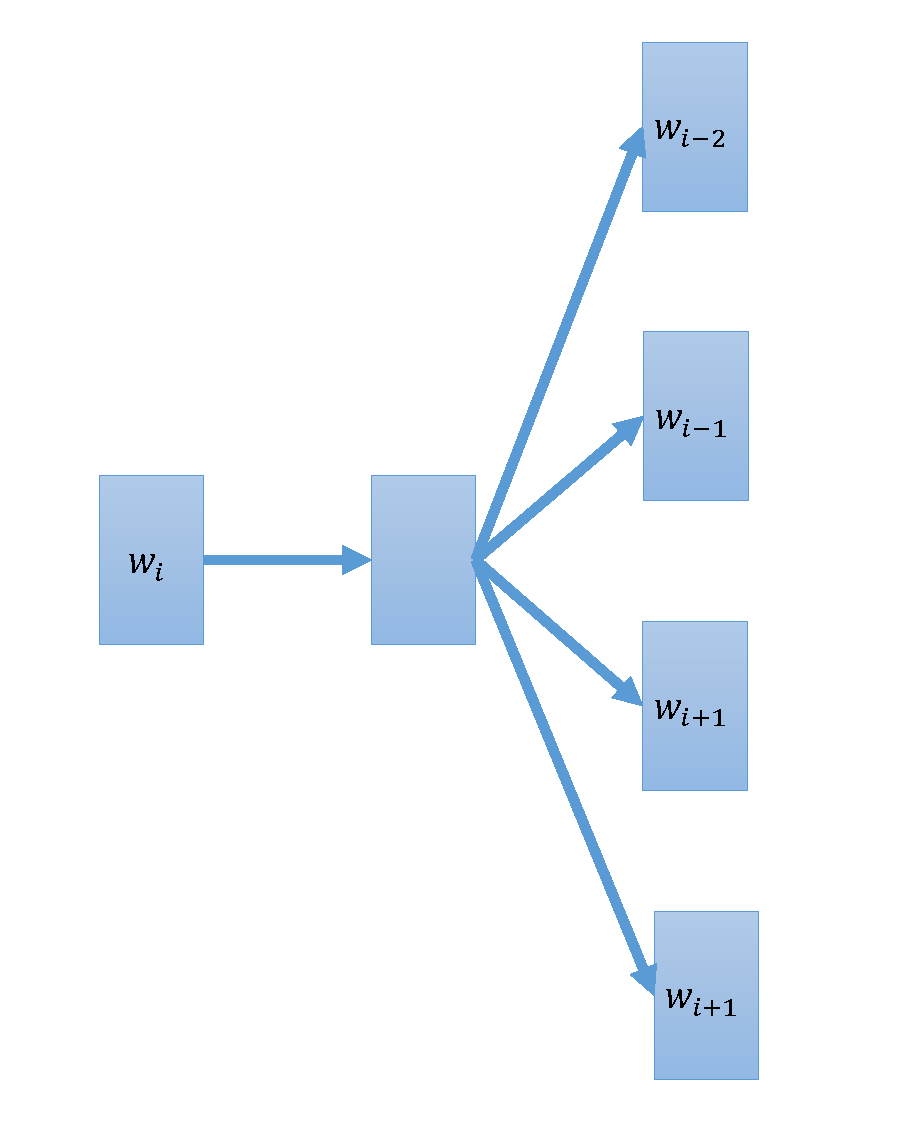
\includegraphics[width=7cm]{skip_gram}
\caption{当$n=4$时Skip-gram网络结构示意图}
\label{fig:skip_gram}
\end{figure}

如\ref{fig:skip_gram}所示,Skip-gram模型由一个两层的神经网络组成,第一层通过$w_i$计算它对应的词向量$\vvec_i$,第二层通过soft根据获得的词向量预测$w_i$的上下文,即$w_{i-2}, w_{i-1}, w_{i+1}, w_{i+2}$。需要注意的是,Skip-gram模型并不考虑上下文所包含词语的顺序,即它将上下文当作一个集合,而不是列表。具体来说,Skip-gram模型的目标函数为:
\begin{eqnarray*}
\sum_{w_i \in D} \sum_{-\frac{n}{2}\leq j \frac{n}{2}} \mathrm{log}P(w_{i+j} | w_i)
\end{eqnarray*}
其中$P(w_{i+j} | w_i)$表示了由一个词语预测其上下文的概率模型。原始版本的$P(w_{i+j} | w_i)$是通过soft-max函数实现的: 
\begin{equation}
\label{eq:soft_max}
P(w_O | w_I) = \frac{e^{{\vvec'_O}^\top \vvec_I}}{\sum_{j \in W} e^{{\vvec'_j}^\top \vvec_I}}
\end{equation}
其中$w_i$与$w'_i$分别表示输入与输出的词向量表示。事实上这个原始的soft-max版本并不能很好得直接运用在实际运算中。是在因为一般情况下,字典中都会包含有较大量级个数的词语,而原始的soft-max的梯度计算的开销是正比于词向量中变量的个数的总和的。我们会在后面看到,\emph{word2vec}使用了两种可以以较高效率进行计算的soft-max的简化与近似。

\subsubsection{CBOW模型}

\begin{figure}
\centering
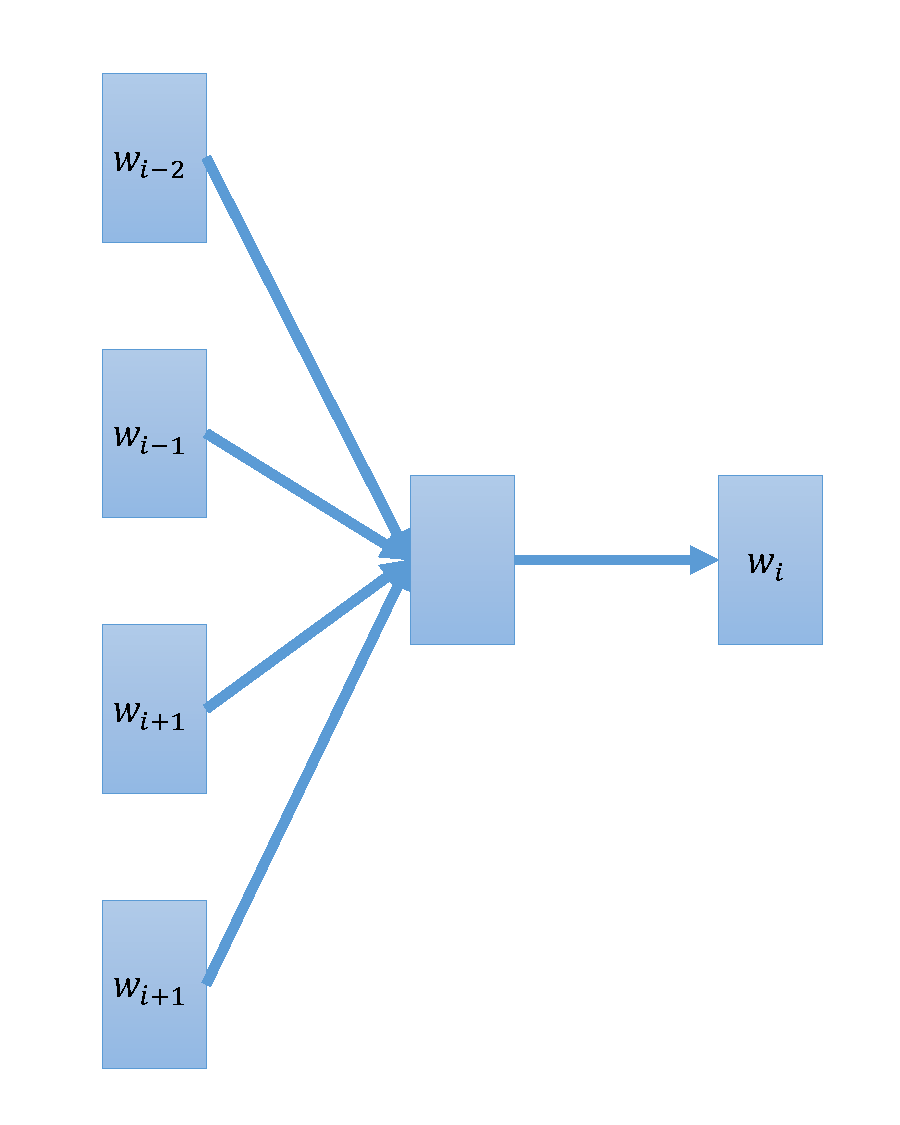
\includegraphics[width=7cm]{CBOW}
\caption{当$n=4$时CBOW网络结构示意图}
\label{fig:CBOW}
\end{figure}

CBOW模型区别于Skip-gram模型之处在于,它是通过根据一个词的语言环境/上下文预测这个词来训练词向量的。

CBOW模型是一个词袋模型,具体来说,它将第$i$个词的周围n个词看作一个词袋,即只关心词语是否在某个词袋中出现,而不关心它们在这个词袋中出现的位置与顺序。

与skip-gram模型类似,CBOW模型同样是一个两层的神经网络,如\ref{fig:CBOW}所示,第一层将某个词语的上下文的词语转化为对应得向量并将它们的和作为上下文对应的语言环境向量,第二层根据这个语言环境向量预测这个词语到底是哪一个。它的目标函数为:
\begin{eqnarray*}
\sum_{w_i \in D} \mathrm{log}P(w_{i} | \sum_{-\frac{n}{2}\leq j \leq \frac{n}{2}} \vvec_{i+j})
\end{eqnarray*}

其中的函数$P(w_{i} | \sum_{-\frac{n}{2}\leq j \leq \frac{n}{2}} \vvec_{i+j})$类似于式\ref{eq:soft_max},也是soft-max函数,这里就不再赘述。

\subsection{Hierarchical Softmax与Negative Sampling}

如上文所说,如果直接使用soft-max函数计算$P(w_O | w_I)$会带来性能上的缺陷与瓶颈。为了简化计算,\emph{word2vec}提出了两种近似方式:Hierarchical Softmax与Negative Sampling。我们下面分别对它们进行介绍。

\subsubsection{Hierarchical Softmax}
\label{subsubsec:HS}

原始的soft-max函数,即使只需要计算某个词语出现的概率,都要使用包含在$W$中的每个词语对应的词向量(共$|W|\cdot N$个变量)来计算soft-max函数的归一化分母,这需要进行大量的运算。实际上,soft-max函数中运算需求最大的地方就是归一化分母部分的计算。

为了简化soft-max,最直观的思路就是改变soft-max的计算方式,使得它的归一化不需要非常大量的计算。\cite{morin2005hierarchical}使用名为Hierarchical Softmax的树状的结构网络,改变了soft-max的计算方式,使之只需要约$\mathrm{log}_2(|W|)$个维度为$N$的向量既可计算出某个词语出现的概率。

具体来说,这个网络将字典中的词语进行编码,并将对应的二叉编码树的结构移植到输出层。这时,该模型假设输出层的每个叶子节点都代表一个词语,而由根节点出发的随机游走最终到达某叶子节点的概率就等于对应词语出现的概率。比如说,对于单词$w$,由于网络的输出层为一棵二叉树,所以有且仅有一条从根节点出发的路径可以到达$w$对应得叶子节点。我们将从根节点出发的这条路径的长度记为$L(w)$,路径上的第$j$个点记为$n_w^j$,其中$n_w^1$为root, $n_w^{L(w)}$为w。则由hierarchical softmax计算出的$P(w_O | w_I)$为:
\begin{equation*}
\label{eq:HS}
P(w | w_I) = \prod_{j = 1}^{L(w) - 1} \sigma(\mathrm{if}(n_w^{j+1} = \mathrm{ch}_{(n_w^j)})\cdot {\vvec'_{n_w^j}}^\top \vvec_{w_I})
\end{equation*}
其中$\sigma(x) = \frac{1}{1+e^{-x}}$为sigmoid激励函数,$if(x)$在$x$为真时为1,$x$为假时为-1,$\mathrm{ch}_n$为n的一个子节点。通过证明,我们知道,上述的定义满足:$\sum_{w \in W} P(w | w_I) = 1$。即在使用上述定义计算$P(w | w_I)$时,不需要额外进行归一化的计算。这使得hierarchical softmax的函数及微分计算均正比于$L(w_O)$,而不是$|W|$。

\subsubsection{Negative Sampling}
\label{subsubsec:NS}

除去Hierarchical Softmax,另一种\emph{word2vec}所介绍的对于soft-max进行简化的方式被称为Negative Sampling。类似于\ref{sec:senna}中所介绍的SENNA模型,由于\emph{word2vec}实际上并不关心skip-gram模型或CBOW模型所进行预测的准确度,而是希望通过它们,可以学习到具有高质量的词向量。Negative Sampling就是基于soft-max函数设计出的一种可以度量词向量质量的函数。它将基于soft-max的目标函数中的$\mathrm{log}P(W_{O}|W_{I})$替换为:
\begin{equation*}
\label{eq:NS}
\mathrm{log}\sigma({\vvec'_{w_O}}^\top\vvec_{w_I}) + \sum_{i = 1}^k \mathbb{E}_{w_i \sim P_n(w)}[\mathrm{log}\sigma(-{\vvec'_{w_i}}^\top\vvec_{w_I})]
\end{equation*}

这样的构造可以被理解为先构造负例,然后再试图将正例与负例之间的差异最大化。同时,另一方面,如同我们已经在\ref{sec:word2vecmf}中提到过的一样,这种构造负例的方法,可以被理解为是在一种特殊的信息矩阵上进行矩阵分解。这些分析与讨论也为Negative Sampling提供了理论依据。同时,在验证试验中,\emph{Negative Sampling}也有很好的实际表现。在下面的文章中,我们也将会将\emph{word2vec}及其相关模型作为讨论的重点。
\iffalse

\bibliography{..\\bib\\tex.bib}

\fi

\chapter{对词向量性质的分析}

词向量学习或词向量嵌入在今年能够成为研究热点的原因之一,在于学习到的词向量具有许多很好的性质,其中最引入注意的一条即是,他往往能够通过代数运算反映词语间的关系。同时很奇妙地是,在学习词向量或进行词向量嵌入的过程中,实际上是没有对这个性质进行显式地约束或建模的。这种性质更像是词向量学习的一种很有价值的副产物。下面我们先对词向量的性质进行介绍,再对为什么会出现这条性质进行分析。

\section{对词向量的性质进行介绍}

通过词嵌入模型学习得到的词向量往往会携带部分语义或语法的信息,而这部分信息,可以通过代数运算反映出来。如我们在\ref{chap:intro}举的例子,$\vvec[\mbox{man}]-\vvec[\mbox{woman}] \approx \vvec[\mbox{king}] - \vvec[\mbox{queen}]$,$\vvec[\mbox{Chinese}] + \vvec[\mbox{river}] \approx \vvec[\mbox{Yangtze\_River}]$,由于man与woman之间的关系与king与queen之间的关系类似,均在与性别的不同,同时,Chinese+River所表达语义与Yangtze\_River类似,所以我们可以认为通过代数运算,词向量可以体现出语义的关系。另一方面,我们还可以观察到$\vvec[\mbox{Chinese}] + \vvec[\mbox{river}] \approx \vvec[\mbox{Yangtze\_River}]$,由于类似的原因,我们认为词向量还可以体现出语法间的关系。

为了进一步验证词向量的这条性质,我们使用\emph{word2vec}发布的工具包,并使用维基百科的英文的语料的前一百万个单词训练了200维的词向量,并用这些词向量进行了验证实验。

\subsubsection{表示国家与首都的单词间的语义关系}

\subsubsection{表示单词与其对应最高级间的语义关系}

\section{对词向量的性质的分析与解释}

在\ref{chap:w2v}我们对\emph{word2vec}模型的介绍中,可以发现,\emph{word2vec}模型的假设中并没有涉及到对词向量间代数运算的说明,也无法保证对词向量进行向量加减会得到有意义的结果,可是,实际上,如同我们在上一节所展示的那样,对\emph{word2vec}所学习获得的词向量进行加减,往往是可以获得有意义的结果的。这是为什么呢?我们将在这一节对这一问题进行简单的探讨与分析。

\section{对词向量的差的分析与解释}

\begin{longtable}{lcccc}
% 首页表头
\caption[词语同时出现概率及比例]{在维基百科的前100万单词中统计的到的单词对同时出现概率及其比例} \label{tab:CoProbRatio} \\
\toprule[1.5pt]
概率与比例 & gas & solid & water & fashion\\
\midrule[1pt]
$P(k|ice)$	&$1.504\times10^{-4}$	&$2.406\times10^{-4}$	&$3.248\times10^{-3}$	&$3.008\times10^{-5}$	\\
$P(k|steam)$	&$4.940\times10^{-4}$	&$5.488\times10^{-5}$	&$2.799\times10^{-3}$	&$5.488\times10^{-5}$	\\
$P(k|steam)/P(k|ice)$	&$3.285$	&$0.228$	&$0.862$	&$1.824$	\\
\endfirsthead

\end{longtable}

\cite{pennington2014glove}中提到,对于具有特定关系的一对词语来说,如ice与steam这两个热力学词语,他们之间的关系,可以通过大量的其他词语分别与这两个词语同时出现的概率来确定。如对于ice与steam,我们选取了4个词语,solid,gas,water,fashion,并把他们与ice和steam同时出现的概率及其比率汇总在表\ref{tab:CoProbRatio}。这四个词中,很明显solid和gas是对这两个词有偏向性的(solid更与ice有关而gas更与steam有关),而water与fashion则是与他们间的关系是无关的(water与这两个词都有关系,fashion与这两个词都没关系)。在这种情况下,ice与steam间的关系可以描述为,使得一个东西与gas变得更相关,与solid变得更不相关。另一方面,表格中的内容也恰好反映出了这一关系。即gas与ice和steam同时出现的概率之比远大于1,而solid与ice和steam同时出现的概率之比远小于1,同时water与fashion同ice和steam同时出现的概率之比均约等于1。

基于此,\cite{pennington2014glove}提出可以通过对词语同时出现的比例进行建模,即构造函数使得$f(\vvec_i, \vvec_j, \vvec_k)$并使函数值尽可能逼近$\frac{P(w_i|w_k)}{P(w_j|w_k)}$。最后提出了新的模型并取得了不错的实验结果。在这里,我们更关系的是为什么通过\emph{word2vec}学习得到的词向量间的差可以反映对应词语见的关系,所以我们对\citep{pennington2014glove}所提出模型的细节不做过多讨论,而将注意力放在对\emph{word2vec}模型的解释上。

如上文所说,在某种程度上,$\frac{P(w_i|w_k)}{P(w_j|w_k)}$的对所有的$w_k \in W$的取值可以反映出$w_i$与$w_j$间的关系。同时,对于一个由\emph{word2vec}训练得到的词向量$\vvec$,我们假设\emph{word2vec}模型中通过上下文预测对应词语或通过对应词语预测上下文均可以获得非常准确的结果,即$f(\vvec_i, \vvec_j) \approx P(w_i|w_k)$,此时$\frac{P(w_i|w_k)}{P(w_j|w_k)}\approx \frac{f(\vvec_i, \vvec_k)}{f(\vvec_j, \vvec_k)}$而在\emph{word2vec}的模型中,$f(\vvec_i, \vvec_j) = \frac{e^{{\vvec'_i}^\top\vvec_k}}{\sum_{w_l \in W}e^{{\vvec'_l}^\top\vvec_k}}$,此时有:
\begin{equation*}
\frac{P(w_i|w_k)}{P(w_j|w_k)}\approx e^{{\vvec'_i-\vvec'_j}^\top\vvec_k}
\end{equation*}
即对于$w_i$与$w_j$,反映它们之间关系的比值可以由他们的对应的词向量的向量差近似得进行逼近。进一步,我们可以说词向量之间的向量差的结果可以表示他们对应词语间的意义。

\section{对词向量的和的分析与解释}

在上一节,我们对$\vvec[\mbox{man}]-\vvec[\mbox{woman}] \approx \vvec[\mbox{king}] - \vvec[\mbox{queen}]$的现象出现的原因进行了讨论,下面我们对$\vvec[\mbox{Chinese}] + \vvec[\mbox{river}] \approx \vvec[\mbox{Yangtze\_River}]$出现的原因进行讨论。

直观上,加法的意义应该对词义有类似聚合的叠加的效果,例如Yangtze\_River是Chinese的最著名的River,所以他可以视为Chinese与River的语义的叠加。但是为什么有这种现象出现呢?

在我看来,如果$w_i$与$w_j$的语义/语法的叠加可以替代$w_k$,那么,对于$w_k$出现的上下文,如果将$w_k$换成包含$w_i$,$w_j$的序列应该也是符合语义/语法的,即:$P(w_k|某种上下文) \approx P(w_iw_j|某种上下文)$,同时
\iffalse

\bibliography{..\\bib\\tex.bib}

\fi

\chapter{针对多义词的语义强化模型及相关实验}

多义词是指同一个词语往往会在不同的语言环境下表达出不同的意义,如词语bank既可以表示银行的意思,也可以表示河岸,在这种情况下,如果我们使用传统的词向量嵌入模型进行词向量的学习,则需要用一个词向量表达多个意思,即忽略了一个词语多个不同的意义之间的区别。

在\citep{bengio2006neural}提出了这个问题后,如我们在\ref{sec:intro_poly}中介绍的,\citep{huang2012improving}通过使用K-Means聚类方法对词语的上下文进行聚类的方式,对一个词语的多个不同意义进行区分后再进行词向量的学习。但是,这个方法需要对多义词的语义数量进行预先指定,即假设每个词语都具有某个固定数目的不同意义。这样的处理方法虽然简化了计算与模型设计,但是同时也使得计算出的词向量可能出现冗余,例如,假设将多义词的不同语义的数量指定为10,则对于一个即使没有多个不同意义的词语,这个模型也会生成10个不同的词向量来表示他的语义。下面,我们对这一方法进行进一步的改进,使得改进后的模型可以对不同的词语产生数量不同的词向量。

原有的方法无法动态地指定词向量的数目的主要原因是他使用了K-Means算法来对上下文进行聚类,而K-Means的聚类算法,是需要指定类的个数的。这个限制使得原有的模型必须要预先对语义数目进行指定。在我们的方法中,我们将K-Means聚类算法替换为层次聚类(Hierarchical Clustering)\cite{johnson1967hierarchical}的方式,这个聚类算法不需要显示地指定类别的个数,而是可以通过其他参数来对聚类所得到的类簇数目进行控制。下面我们先对层次聚类进行简单的介绍,再来详细说明我们改进后的算法。

\section{层次聚类}

\begin{figure}
\centering
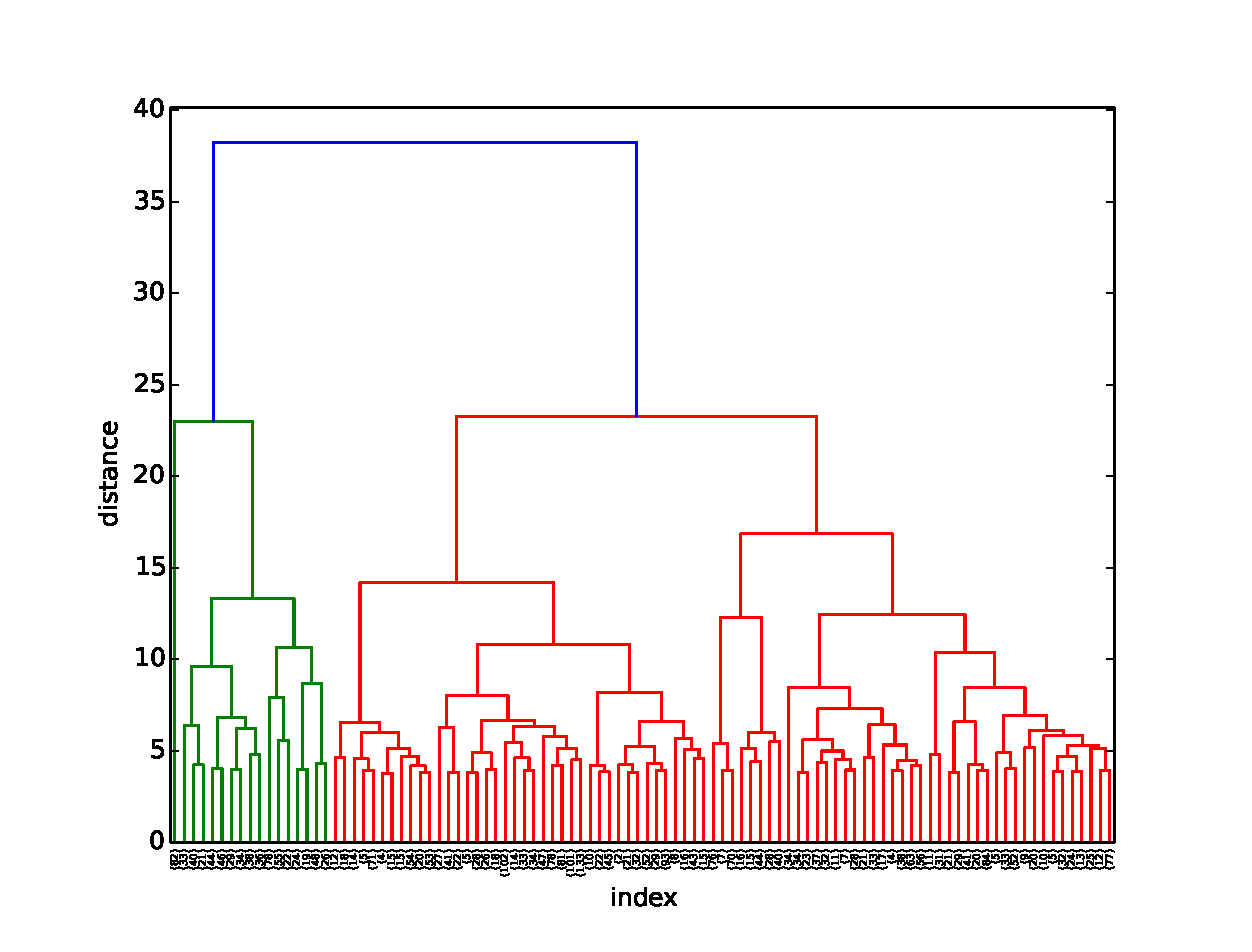
\includegraphics[width=13cm]{hs}
\caption{层次聚类示意图}
\label{fig:hs}
\end{figure}

层次聚类是一种聚类方法,这种方法通过建立树状体系的类簇结构来进行聚类。如图\ref{fig:hs}所示,层次聚类最后得到的结果也不是单独的类簇标号,而是一棵表示类簇结构的树。这种做法的好处在于不需要在聚类的时候对类簇的个数进行限定,在获得这样一棵树之后,在树的任意高度进行分割,就可以获得最后的聚类结果。例如,在图\ref{fig:hs}中高度为30处进行分割,将会得到两个类簇,即左边以绿色标注的类簇,以及右边以红色标注的类簇。

一般来说,层次聚类分为两种,一种是自底向上,另一种是自顶向下。其中,自底向上的算法在最开始将每一个点都视为一个独立的类簇,然后迭代得将两个距离最近的类簇合并为一个类簇,直到只剩下一个类簇,同时,这个逐次合并的过程就会被作为层次聚类所得到的树形结构记录。类似地,自顶向下的方法是在最开始将左右的点都视为同一个类簇,然后通过迭代每次将一个类簇划分为两个类簇,并将这个逐次划分的过程进行记录。

\section{使用层次聚类方法学习多义词对应词向量的算法}

根据\emph{The Distributional Hypothesis},我们知道,当一个多义词以不同的词义出现时,他的上下文应该有所不同。基于这一点,我们可以先对一个词的上下文进行计算并记录,然后再对这些上下文进行聚类,并按照聚类的结果对多义词的语义进行区分。在区分出多义词的多个语义后,我们可以将一个词语的不同语义当成不同词语,然后使用传统的词向量嵌入算法进行词向量的学习。下面我们按照顺序进行介绍。

\subsection{对词语上下文的计算}

一个词语出现的上下文可以被直观描述为词语周边的其他词语的集合,在这里,类似于\citep{huang2012improving},我们将这些词语的加权和作为一个词语的上下文。即先使用\emph{word2vec}工具包计算出词向量,然后对于每个词语,对他周围词语的词向量进行加权求和,并将求和后的向量作为这个词语这一次出现的上下文,即对于语料中的一个词语序列:$w_{i-n}, \cdots,w_{i}, \cdots, w_{i+n}$,词语$w_i$这次出现的上下文为:$\sum_{j \in [-n, n]} \vvec_{i+j} \cdot a_{i+j}$,其中$a_{i+j}$为权值,并满足$\sum_{j \in [-n, n]} a_{i+j} = 1$。为了得到更准确的计算结果,我们将没有什么实际含义的功能词(stop words),例如the, on等,对应的权重设为0。然后我们将Inverse document frequency(IDF)值($w$为某个单词,$d$为某篇文档):
\begin{equation*}
\mathrm{IDF}(w, D) = \mathrm{log} \frac{N}{|\{d | w \in d, d \in D\}| + 1}
\end{equation*}
进行归一化后,作为剩余词的权值:
\begin{equation*}
a_{i+k} = \frac{\mathrm{IDF}(w_{i+k}, D)}{\sum_{j \in [-n, n]} \mathrm{IDF}(w_{i+j}, D)}
\end{equation*}

\subsection{对上下文使用层次聚类分辨多义词的不同语义}

\begin{longtable}{lccc}
% 首页表头
\caption[在三种不同的设定下层次聚类所得到的类簇个数]{在三种设定下对表示上下文的向量进行层次聚类后得到的类簇个数}
\label{tab:num4hc} \\
\toprule[1.5pt]
词语 & 类簇个数(设定一) & 类簇个数(设定二) & 类簇个数(设定三) \\
\midrule[1pt]
country	&	5	&	& \\
pear	&	1	&	3	& \\
cell	&	5	&	312	& \\
light	&	11	&	& \\
play	&	15	&	& \\
mark	&	3	&	& \\
fall	&	4	&	& \\
head	&	5	&	& \\
close	&	12	&	& \\
\endfirsthead
\end{longtable}

在完成表示词语上下文的计算后,我们通过层次聚类算法来对每个词语的不同意思进行区分。在使用层次聚类时,我们使用了Ward Distance\cite{ward1963hierarchical}作为距离计算的方法。同时,为了使不同的词语具有多样且合理的语义数量,我们选择使用Inconsistency作为划分类簇结果的标准。

下面我们将我们使用的层次聚类常的设定与其他两种设定进行对比,通过实验结果来验证说明我们使用的层次聚类的设定的合理性。我们将我们所使用的设定记为设定一,将对比的两种设定分别记为设定二和设定三。其中,设定二使用一个类簇中的最大距离的上限作为划分类簇的标准,设定三使用。如\ref{tab:num4hc}所示,设定一,
通过与其他设定进行比较,我们对层次聚类的设定使得聚类结果的类簇个数具有较好的多样性与合理性。

\subsection{完成多义词的不同语义辨别后得到的词向量}

\begin{longtable}{cc}
% 首页表头
\caption[与多义词不同语义对应词向量距离最近的词语]{对表示上下文的向量进行层次聚类后得到的类簇个数统计表}
\label{tab:near4demo} \\
\toprule[1.5pt]
词语 & 与该词语最近的五个词语 \\
\midrule[1pt]
fall\_1	& autumn, spring, demise, summer\\
fall\_2 	& falling, disappear, erupt, fade, rebound\\
mark\_1	& 400th, 300th, 500th, fiftieth, 200th\\
mark\_2	& signifying, signify, zodiac, syllable, auspicious\\
country\_1	&	nation, Africa, commonwealth, zoo, comoros\\
country\_2	&	reggae, bluegrass, funk, hip-hop, blues\\
\endfirsthead
\end{longtable}

在通过层次聚类,完成对多义词的不同语义进行判别后,我们现在将一个词的不同语义作为不同词语对待,并通过\emph{word2vec}工具重新学习了词向量。

下面那我们通过实验来说明我们获得的词向量可以对多义词的不同词义进行表示与区分。由于词向量携带部分语义信息,我们选择通过罗列与词向量最近的其他词向量所对应的词语,来展示词向量的所携带的语义信息的种类。我们选择了三个多义词,country,fall,mark的部分词向量进行实验,如表\ref{tab:near4demo}所示,我们可以观察到fall所对应的主要的两个语义,落下与季节,被很好得区分开来,country所对应的国家与音乐种类这两个意义也被很好得区分开来,类似地,mark的语义也在他的两个词向量中得到了区分。这说明我们学习获得的词向量确实可以对多义词的不同语义进行较好地区分与表示。
\iffalse

\bibliography{..\\bib\\tex.bib}

\fi

\chapter{结论}

本文先对现有的词向量嵌入模型进行了总结与分析,讨论了词向量所具有的一些性质与这些性质背后的机制与原理。之后,观察到针对多义词对词向量进行语义增强的方法往往具有无法对多义词的语义个数进行分辨的缺点,我们使用层次聚类的方法对现有的词向量学习算法进行了改进,并通过实验验证了使用层次聚类方法进行多义词不同词义辨别的有效性。
% \input{chapters/figure}
% \input{chapters/table}
% \input{chapters/math}
% \input{chapters/algorithm}
% \input{chapters/code}
% \input{chapters/citation}
\bibliography{bib/tex}

% \appendix
% \chapter{论文规范}

\backmatter
\begin{acknowledgements}

大学的学习生活几乎都是伴随着我的导师徐林莉老师的鼓励、指导与批评度过的。在平时生活中,她不仅在为人处事上给了我许多启示,还叮嘱我注意健康,不让我刷夜;在学业上,她花费了大量的时间与我讨论,指引我、带领我找到、探索有趣的问题,甚至在大年初一还在帮我修改论文,同时她还会督促我注重英语及其他课程的学习,并且在我申请实习以及博士项目的时候鼓励我、帮助我,这一切我都终生难忘,我在这里再次衷心感谢老师对我的淳淳教诲和悉心关怀。

在大四去微软亚洲研究院实习的一年中,谢幸老师与宋睿华老师对我的学习、科研以及申请提供了非常多的指导、鼓励与帮助,他们在我需要GPU时帮我申请计算资源,在我出国申请时帮助我,还与我分享他们的人生经验,这些支持与教导对我来说都是宝贵的财富,衷心感谢老师的帮助与指导。

最后,我要感谢学院以及本科期间所遇到的每一位老师对我的培养与教导;感谢王臻师兄,陈再毅师兄,黄艾青师姐,李亦锬师兄和仲小韦师兄一直以来对知识的无私分享;感谢我的家人一直以来对我的支持,包容与陪伴,你们是我最坚实的后盾。

\end{acknowledgements}

\iffalse

\bibliography{..\\bib\\tex.bib}

\fi


\begin{publications}

\section*{已发表论文}

\begin{enumerate}
\item Liyuan Liu, Linli Xu, Zhen Wang and Enhong Chen, \textbf{Community Detection Based on Structure and Content: A Content Propagation Perspective}, \emph{The 15th IEEE International Conference on Data Mining (ICDM'2015)}: 271-280, Atlantic City, NJ, USA, November 14-17, 2015.
\end{enumerate}

\end{publications}


\end{document}
